%! Author = tstreule

\section{Mechanical Sensors}
%%%%%%%%%%%%%%%%%%%%%%%%%%%%%%%%%%%%%%%%%%%%%%%%%%%%%%
%%%%%%%%%%%%%%%%%%%%%%%%%%%%%%%%%%%%%%%%%%%%%%%%%%%%%%
\subsection{Viscoelastic media}
%
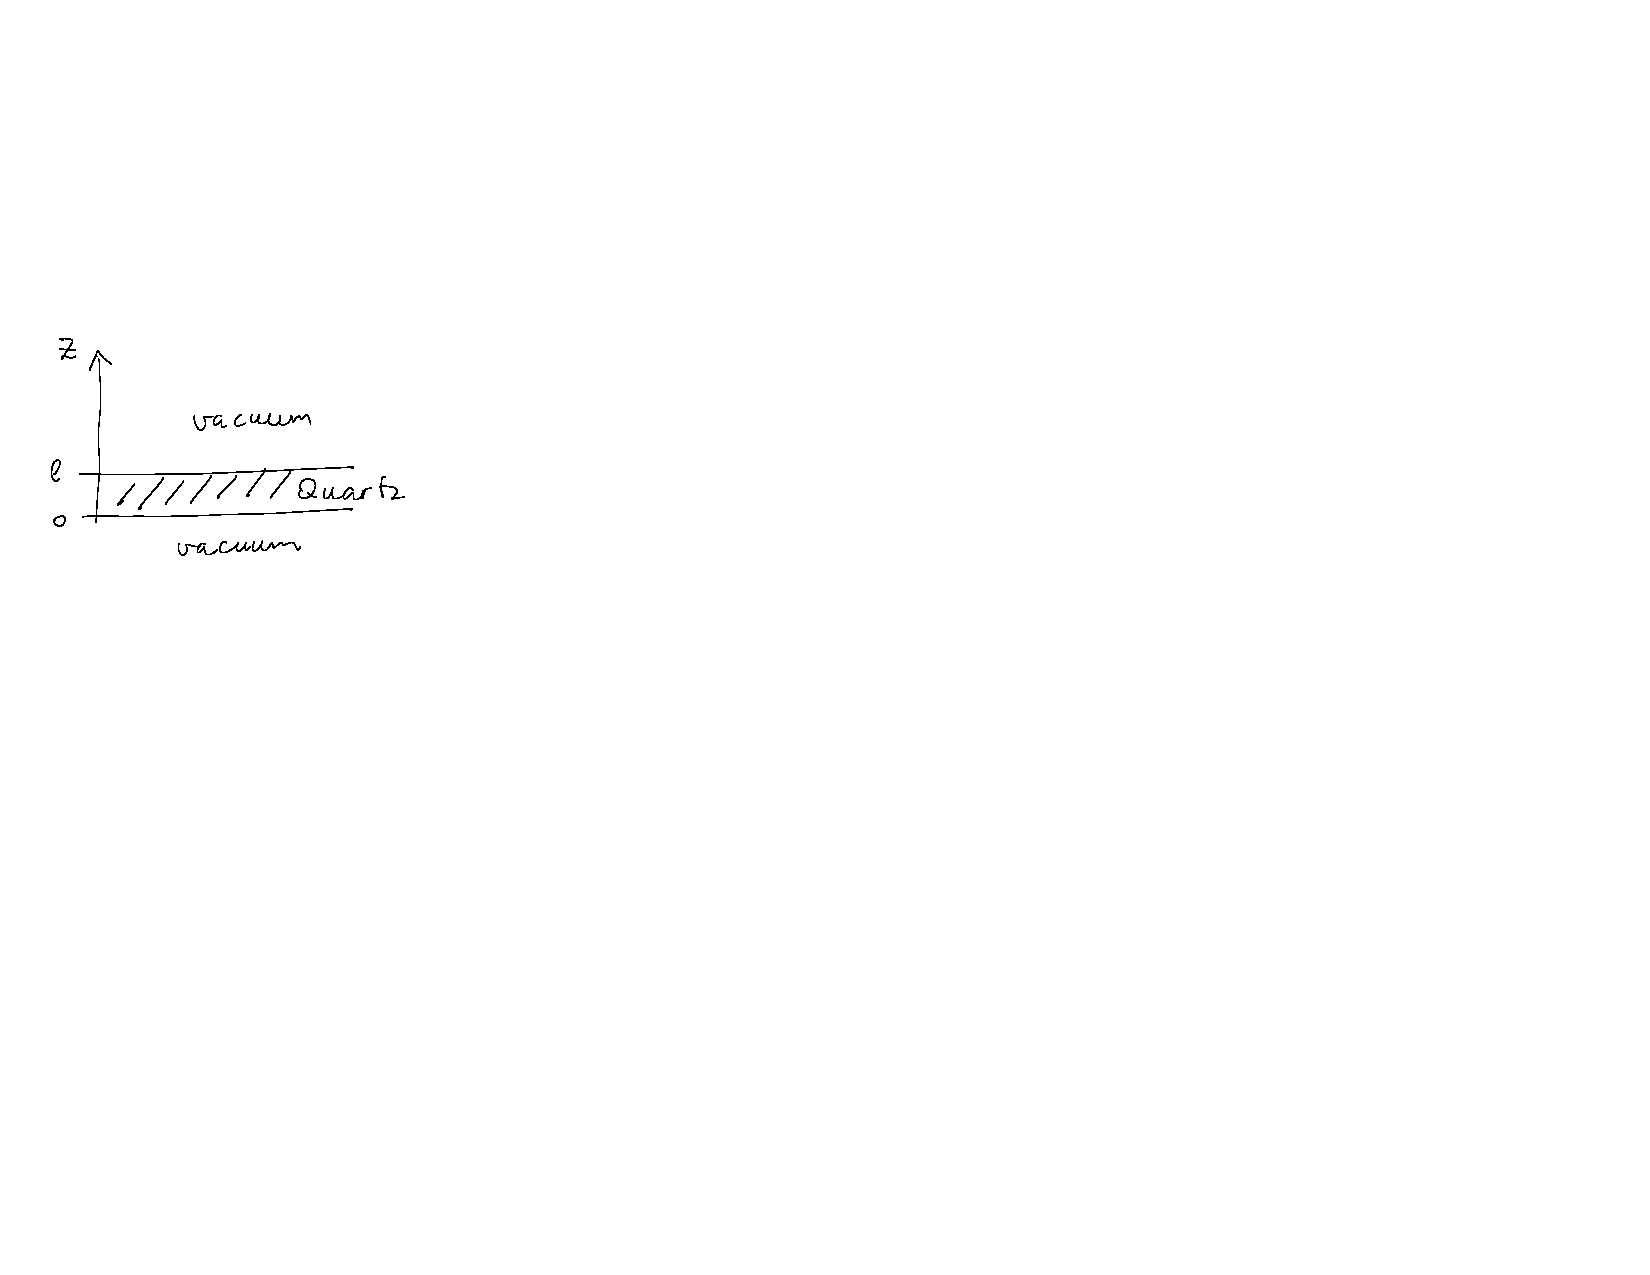
\includegraphics[width=.3\columnwidth]{Mechanical_1}\hfill
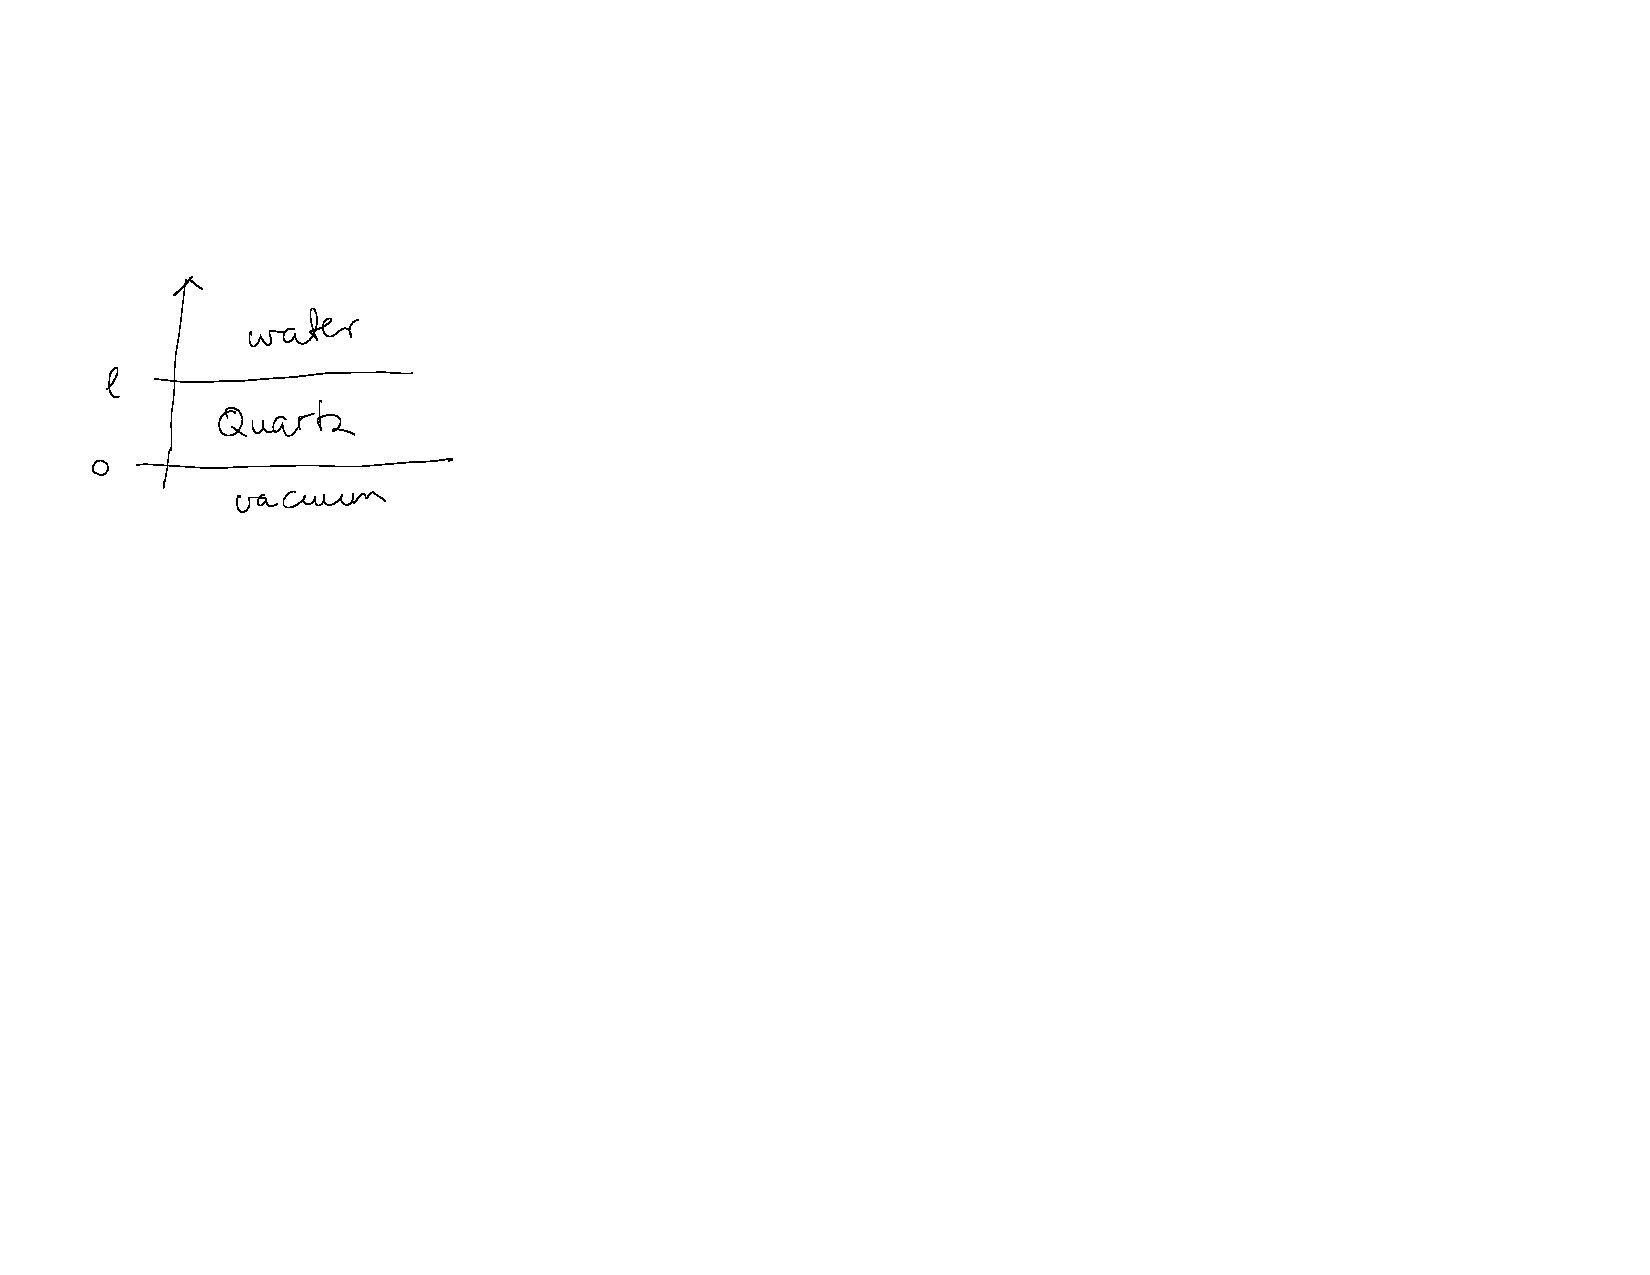
\includegraphics[width=.3\columnwidth]{Mechanical_2}\hfill
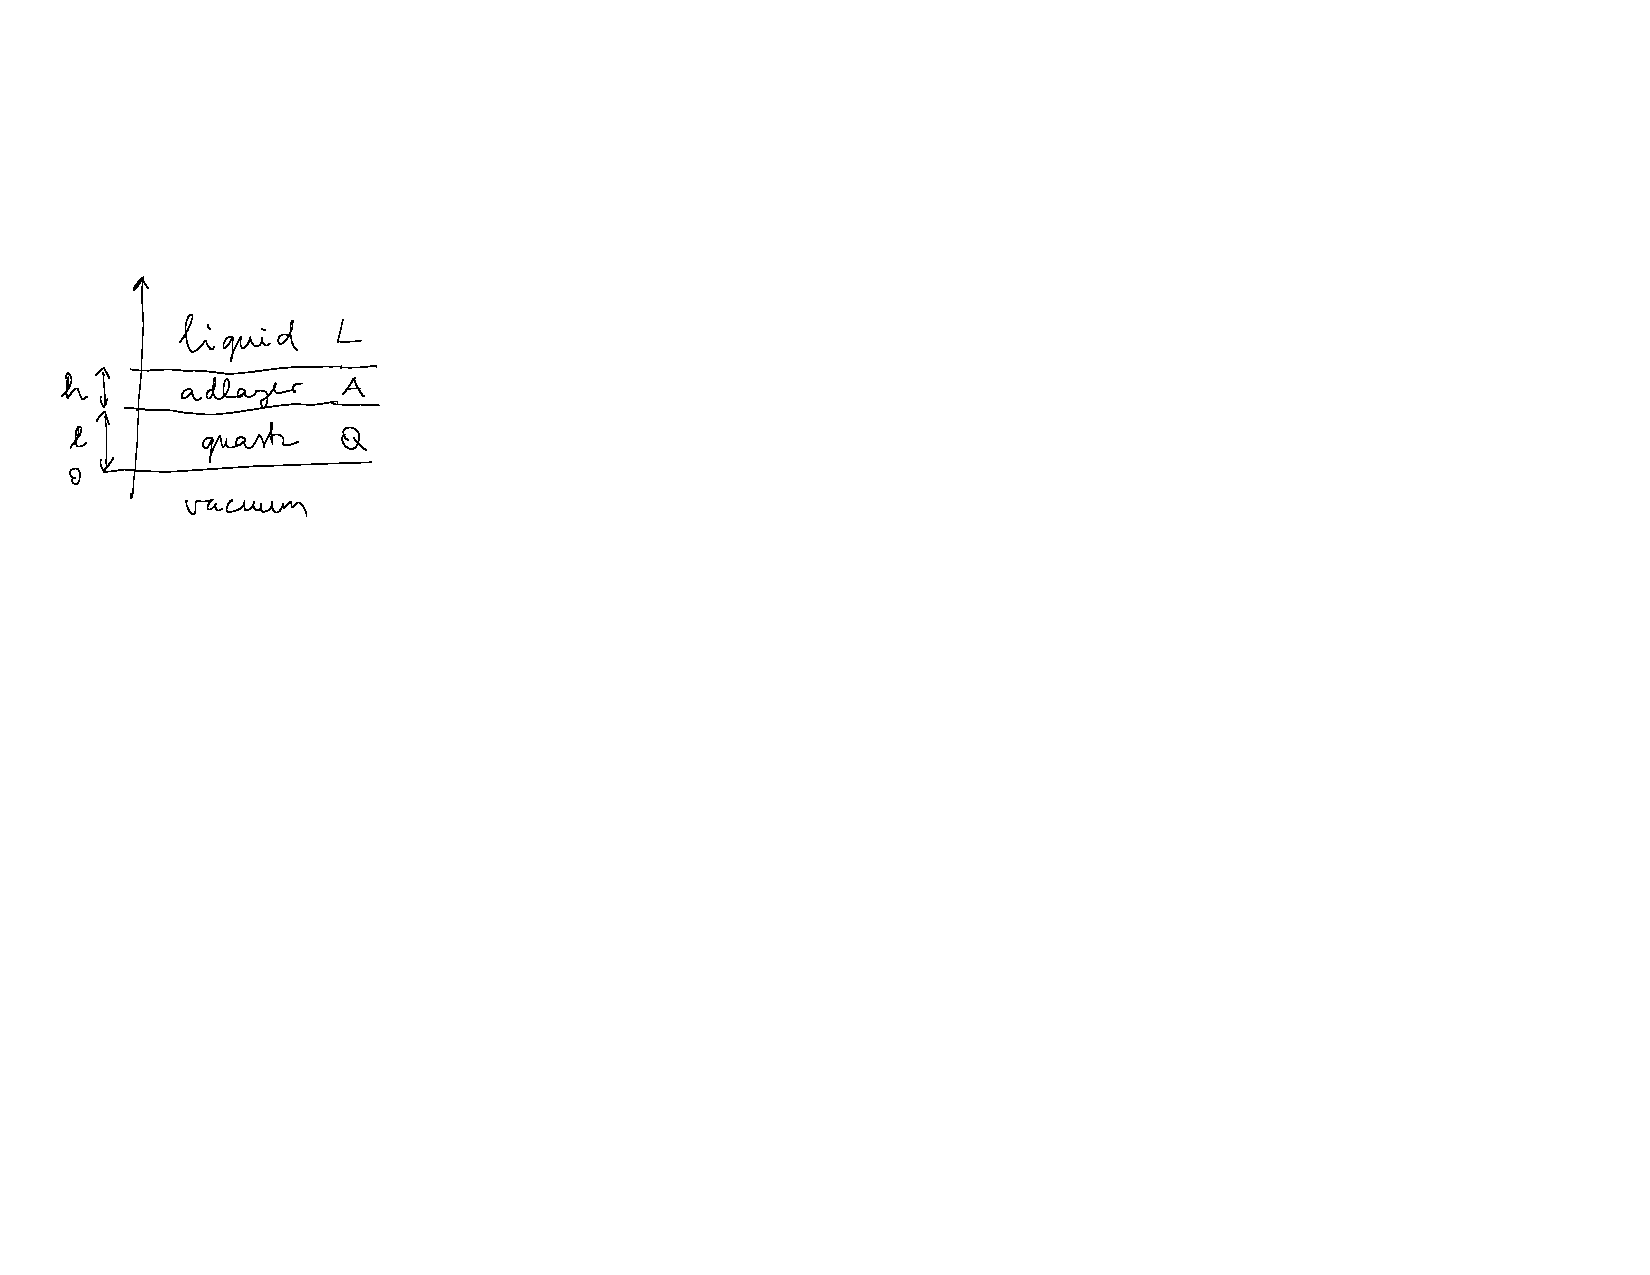
\includegraphics[width=.3\columnwidth]{Mechanical_3}

\textbf{Remark}: Calculate \textit{always} at first in $\unitfrac{rad}{s} \overset{\scriptstyle \times\unitfrac{1}{2\pi}}{\longrightarrow} \unit{Hz}$.
%%%%%%%%%%%%%%%%%%%%%%%%%%%%%%%%%%%%%%%%%%%%%%%%%%%%%%
\subsubsection{Crystal with thickness $l$}
%
\formbox[\unitfrac{rad}{s}]{Resonance frequency}{\omega_n = n\cdot\omega_0 = n\cdot \frac{\pi}{l} \sqrt{\frac{\mu_Q}{\rho_Q}}}
%\formula{overtones}{q\coloneqq \omega\sqrt{\frac{\rho}{\mu}}, \enskip \lambda = 2\pi / q = 2l / n}
\formula{char. wavelength}{\lambda = 2l/n}
%%%%%%%%%%%%%%%%%%%%%%%%%%%%%%%%%%%%%%%%%%%%%%%%%%%%%%
\subsubsection{Elastic plate in water}
%
\formbox{Resonance frequency}{\omega_n = n\omega_0 + \Delta\omega_n}
\formula{frequency shift}{\Delta\omega_n = -\sqrt{n} \,\sqrt{\frac{\rho_L\,\eta_L\,\omega_0}{2}} \frac{1}{l\,\rho_Q} \textrm{,\enskip $\eta_L$: viscosity}}
%%%%%%%%%%%%%%%%%%%%%%%%%%%%%%%%%%%%%%%%%%%%%%%%%%%%%%
\subsubsection{Elastic plate in water with adlayer}
%
In fact is the \textit{resonance frequency} dependent on the adlayer height.\\
But if it is ``enough'' small, the Sauerbrey approx. is sufficient.

\formbox{\textbf{Sauerbrey eq.}}{\!\!\Delta f_n = 2\pi\omega_n = -n\frac{\Delta m}{C}\!\!}
\hfill $C {=}\frac{\sqrt{\rho_Q\,\mu_Q}}{2f_0^2} {=} \unit[17.7]{\!\!\frac{\unit[]{ng}}{\unit[]{cm^2Hz}}}$
%%%%%%%%%%%%%%%%%%%%%%%%%%%%%%%%%%%%%%%%%%%%%%%%%%%%%%
\subsection{QCM-D \textit{vs.} SPR techniques}
%
\begin{tabular}{@{}l @{\qquad}l}
    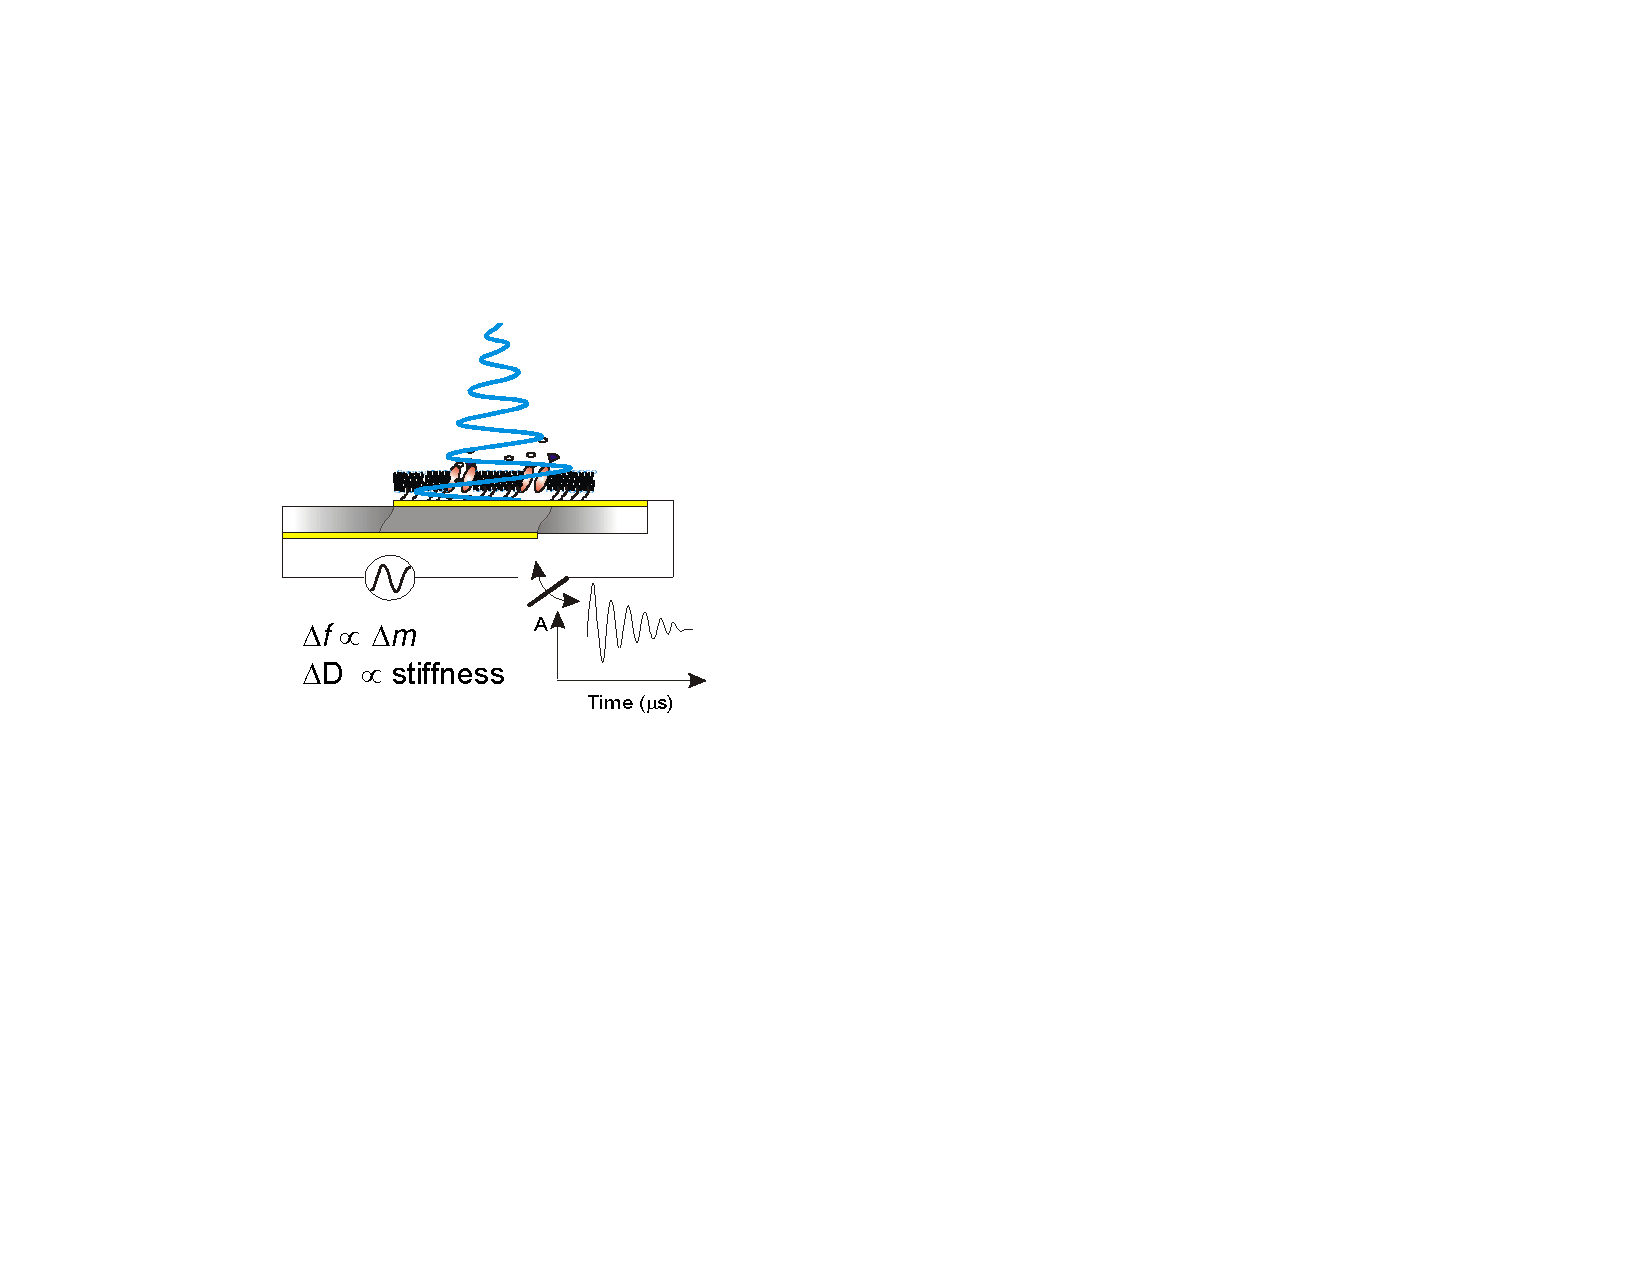
\includegraphics[width=.35\columnwidth]{Mechanical_vs_QCM} &
    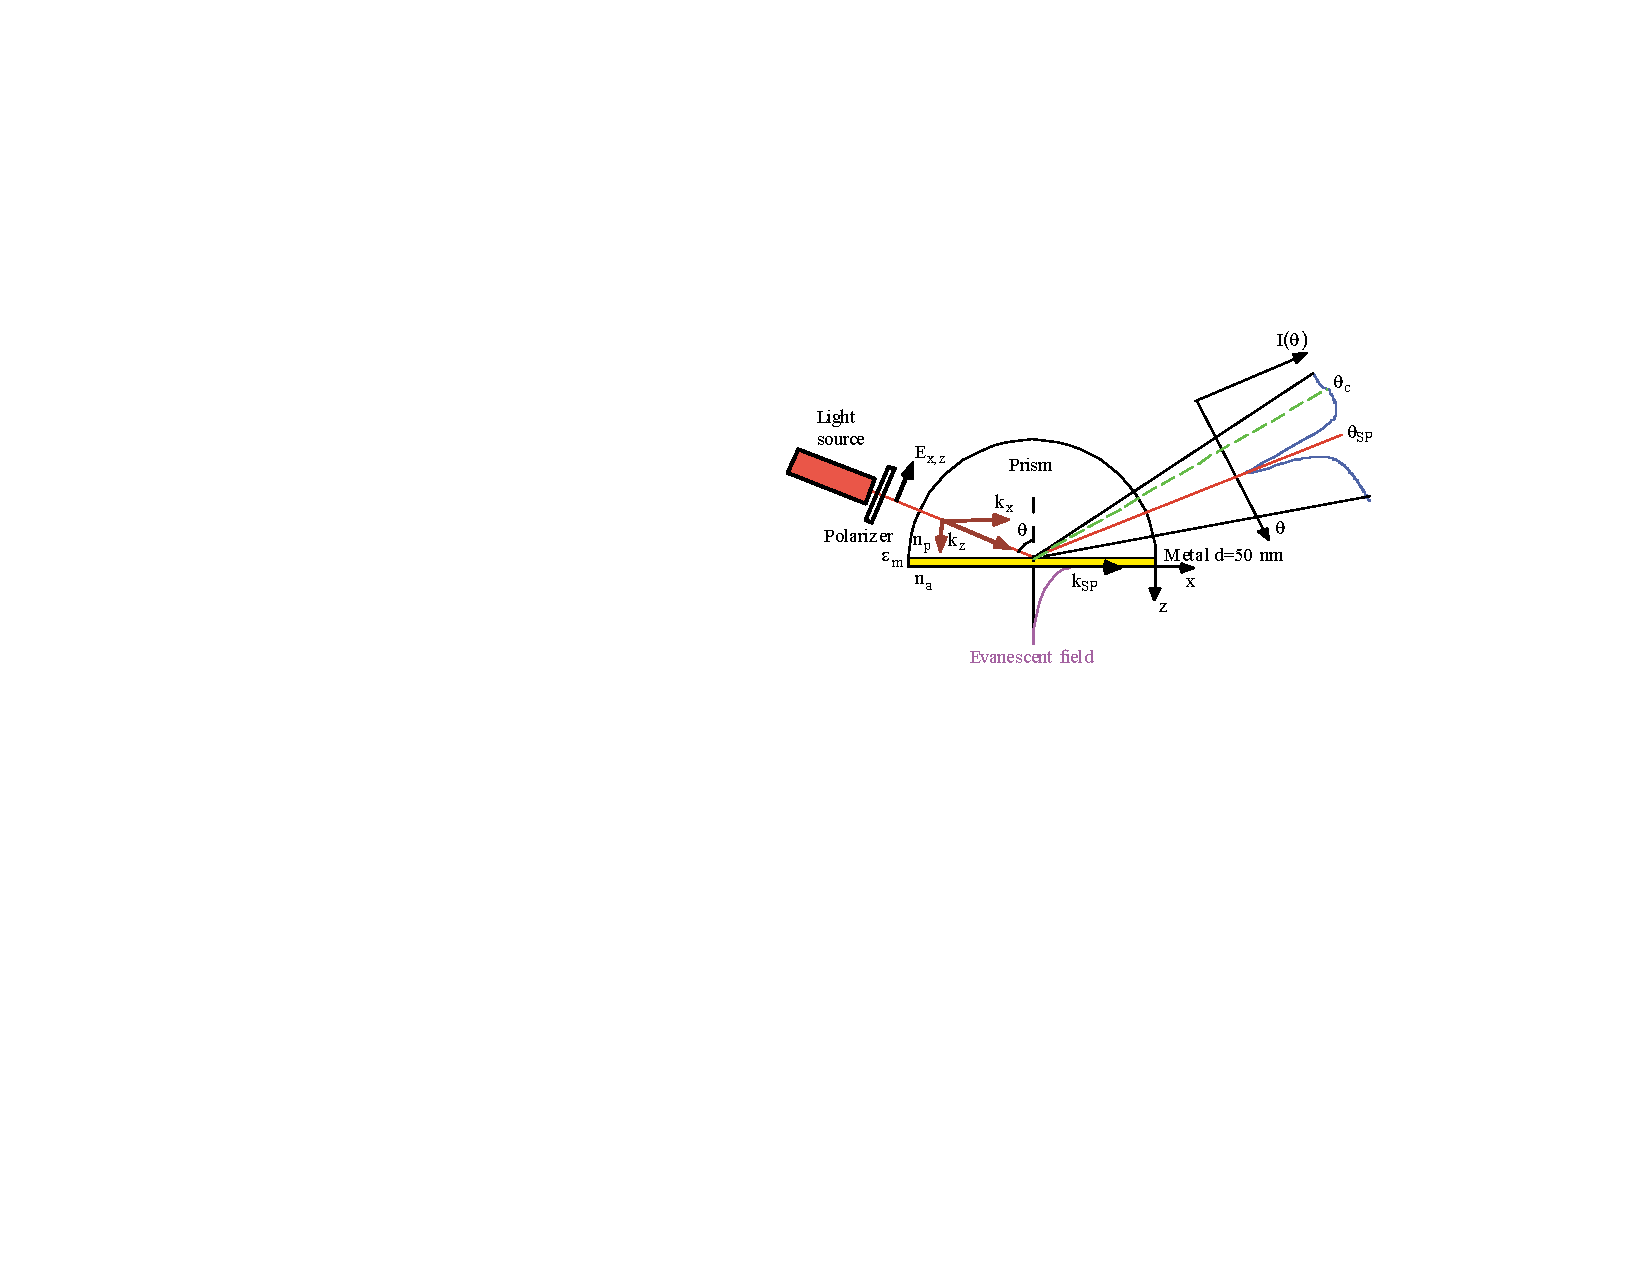
\includegraphics[width=.5\columnwidth]{Mechanical_vs_SPR}
    \\\addlinespace
    \highlight{$\Delta m = -\frac{C}{n} \Delta f_n$} &
    \highlight{$\textstyle \Delta m = d\,\frac{n\ped{protein} - n\ped{buffer}}{\diff n/\diff c}$}
    \\\addlinespace
    $\textrm{LOD}\ped{QCM} = C\cdot \delta f     \simeq \unitfrac[1]{ng}{cm^2}$ &
    $\textrm{LOD}\ped{SPR} = C\cdot \delta\theta \simeq \unitfrac[0.1]{ng}{cm^2}$
\end{tabular}
%%%%%%%%%%%%%%%%%%%%%%%%%%%%%%%%%%%%%%%%%%%%%%%%%%%%%%
\subsection{QCM: Quartz Crystal Microbalance}
%
\formbox{Resonance cond.}{f = \frac{n\,v}{\lambda} = \frac{n\,v}{2t}}
\formula{Dissipation}{D = \frac{1}{\pi f\tau},}
$\tau$: time until $\frac{U\ped{max}}{\eu}$

\vspace{-9mm}
\begin{minipage}{\linewidth}
    \hfill
    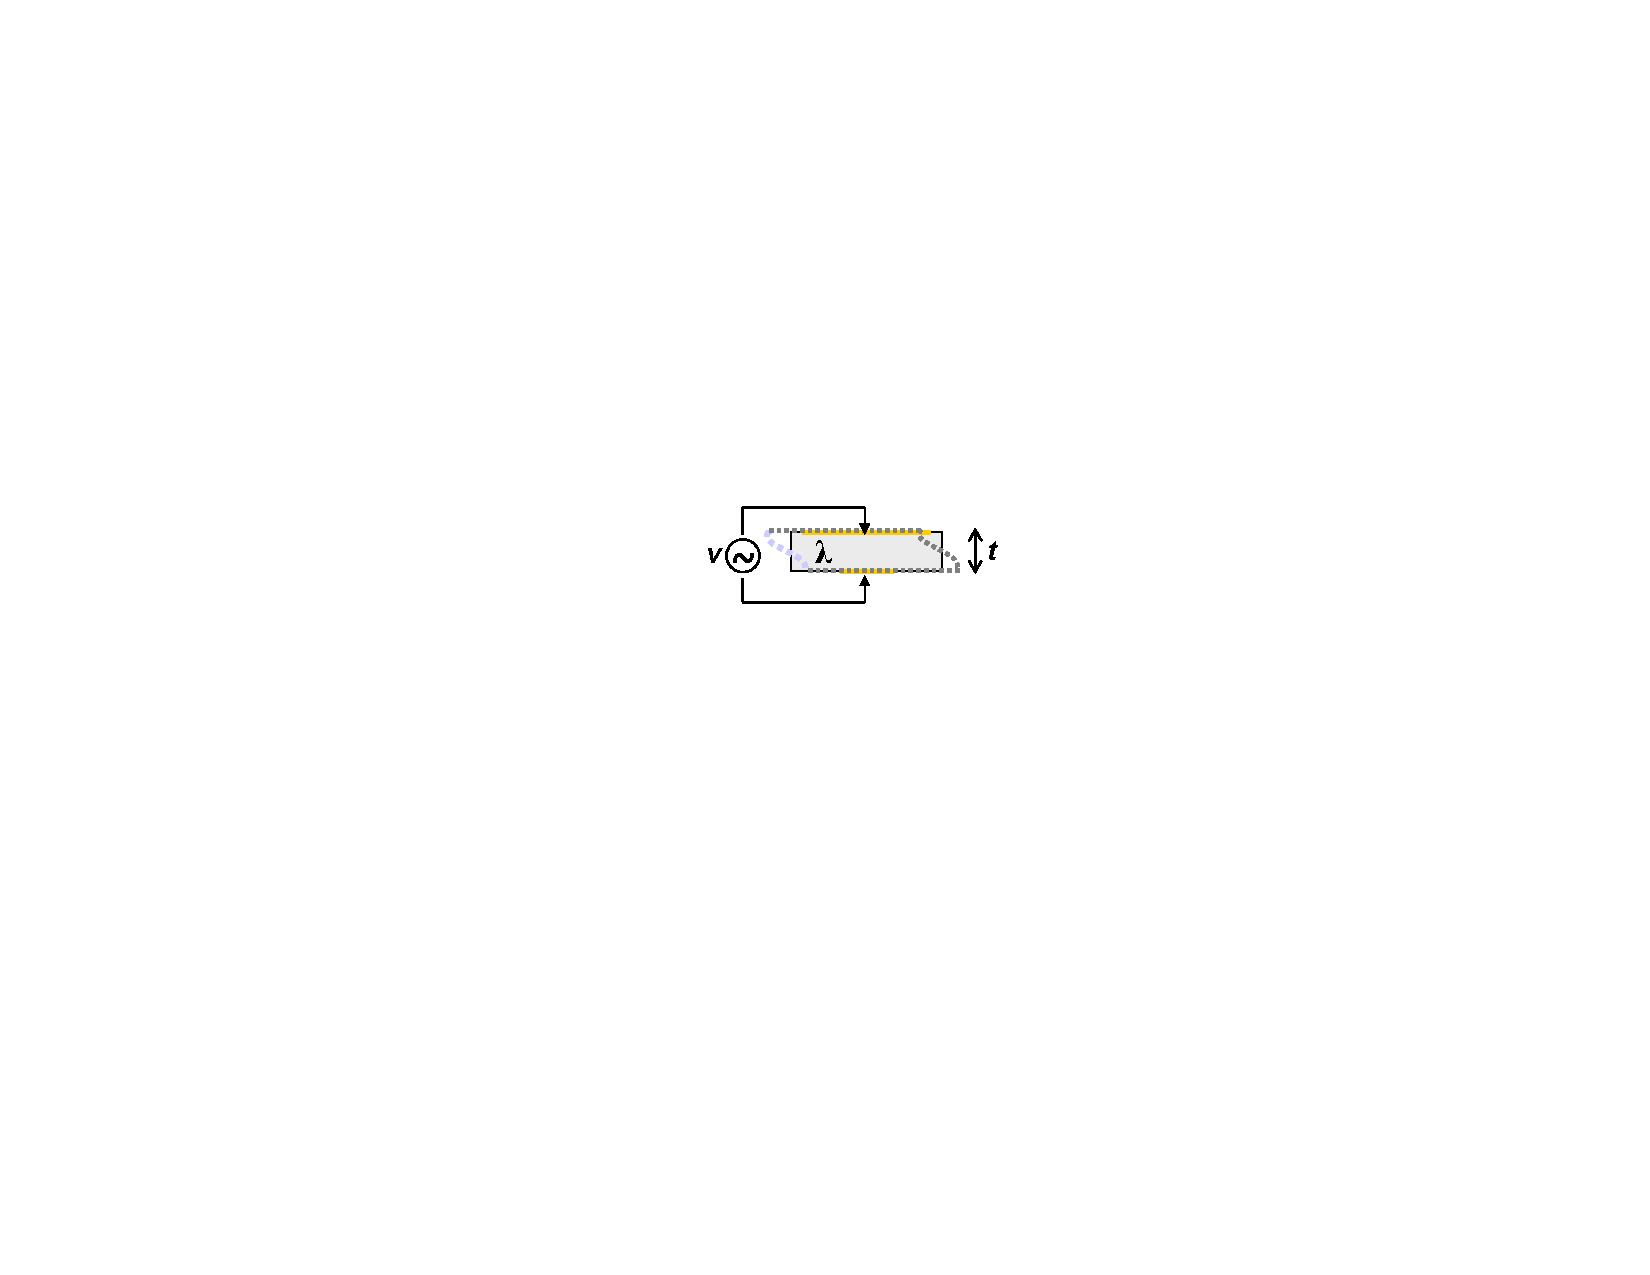
\includegraphics[width=.23\columnwidth]{Mechanical_QCM}
\end{minipage}
\vspace{2mm}

\textbf{Modeling of the QCM-D response} in air / aqueous solution:\par
\begin{minipage}{.25\columnwidth}
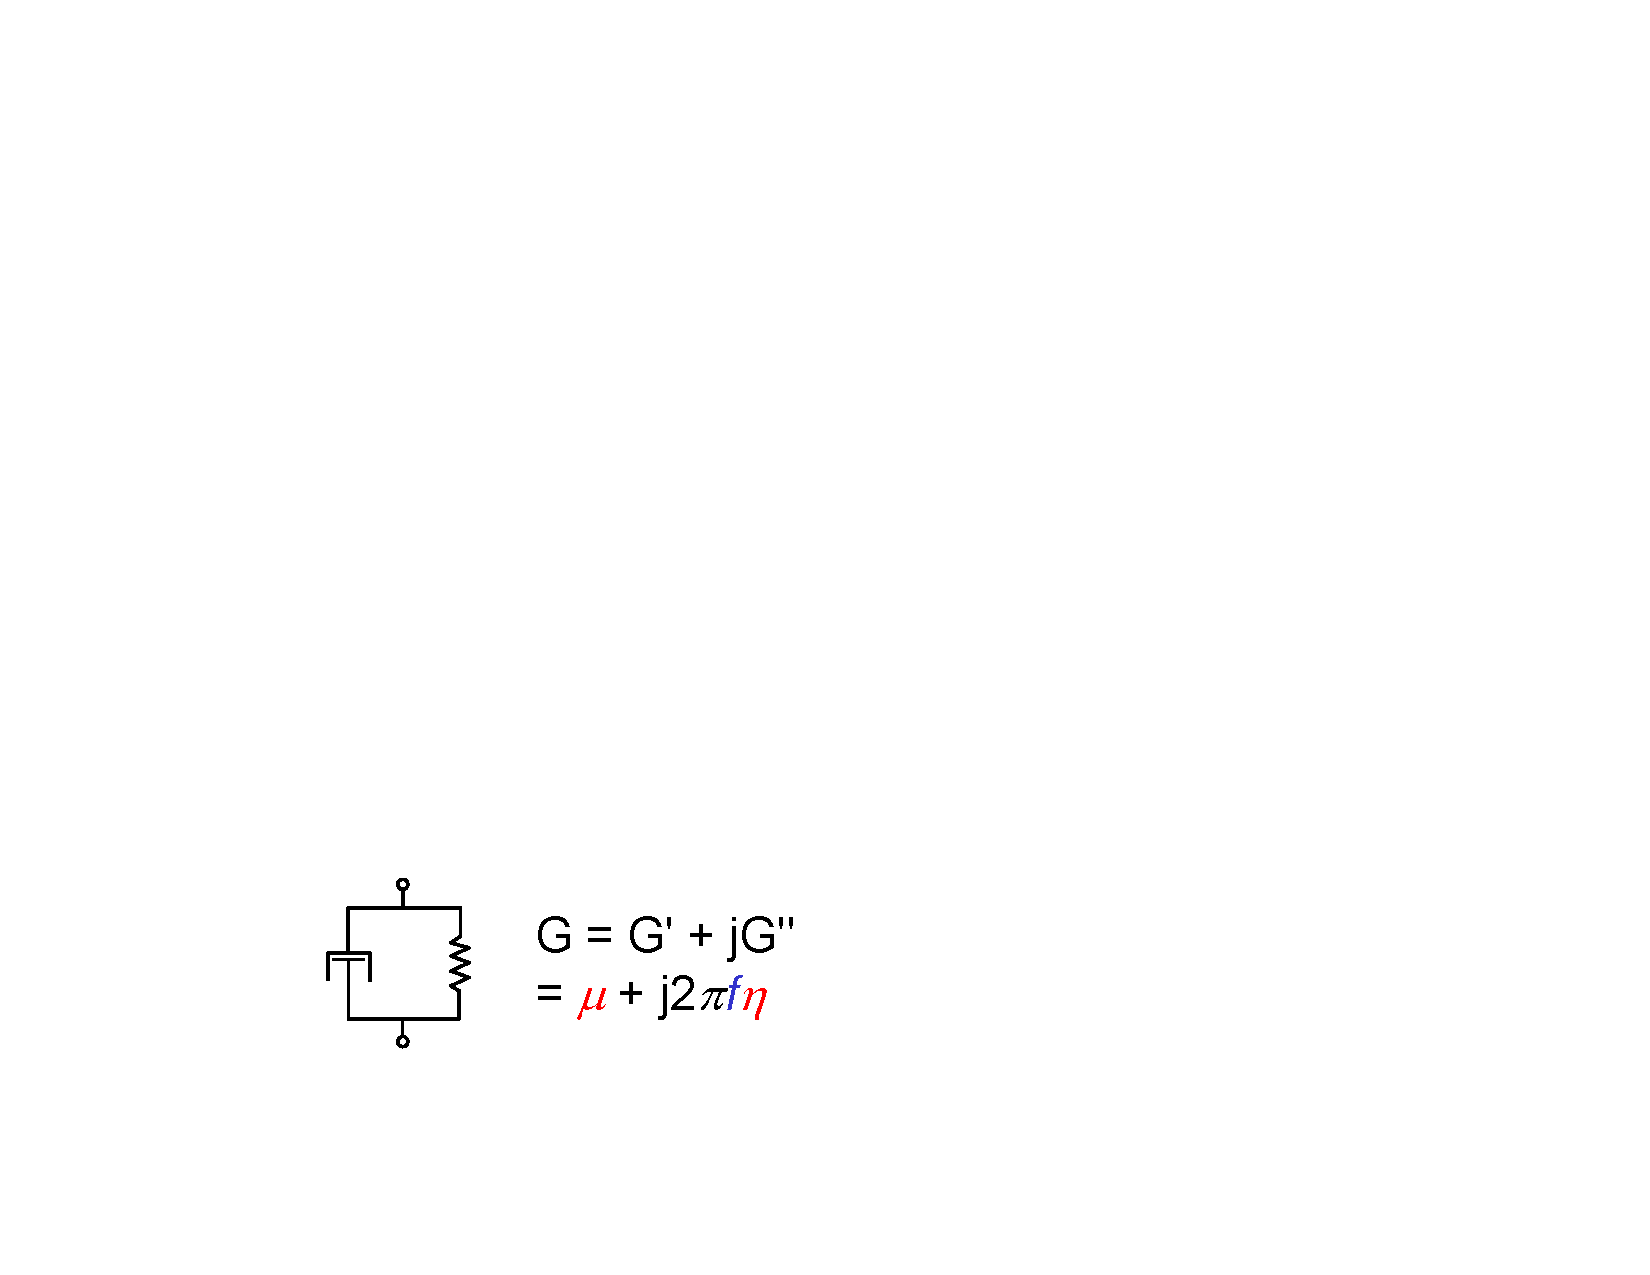
\includegraphics[width=.88\columnwidth]{Mechanical_QCM_Modeling}
\end{minipage}%
\begin{minipage}{.75\columnwidth}
$\eta$: viscosity ($=\frac{G''}{\omega}$), $\mu$: elasticity ($=G'$),\\
$\rho$: density, $d$: thickness
%\formula{Resonance condition}{f = \frac{n\,v}{\lambda} = \frac{n\,v}{2t}}
\end{minipage}
%%%%%%%%%%%%%%%%%%%%%%%%%%%%%%%%%%%%%%%%%%%%%%%%%%%%%%
\subsection{Strain Gauge}
%
\formula{Resistive strain g.}{\frac{\Delta R}{R} = k\,\frac{\Delta l}{l} = k\,\epsilon
\textrm{,\enskip $\epsilon$: Strain, $k$: Gauge factor}}
\formula{Capacitive strain g.}{C = \epsilon_0\epsilon_r\,\frac{A}{d} \textrm{,\enskip (displacement: $d \to d+\Delta d$)}}
